\section{Stochastic structure of magic theories}
\label{sec:struc}

\subsection{Magic fragments}\label{sec:magfrag}

Equipped with the definitions of the Wigner distribution in odd prime dimensions, we can formally recast the maximal magic theory $\Rmax$ into a stochasticity setting.
The free states correspond to proper probability distributions 
\begin{equation}
    \Fmax \coloneqq \{ \rho: \W[\bmz]{\rho} \geq 0 \text{ for all } \bmz \in \pd\}
\end{equation}

The free operations should send the set of free states $\Fmax$ into itself and completely preserve the non-negativity of the states, in the sense that $\E \in \Omax$ iff $(\id_d \otimes \E ) \sigma \in \stab$ for all odd prime dimensions $d$ whenever $\sigma \in \Fmax$.
It is shown by Wang \textit{et al.}~\cite{cit:wang} that $\Omax$ coincides with the set of operations $\E$ that correspond to stochastic Wigner distributions, 
\begin{equation}
    \Omax = \{ \E: \W[\bmy|\bmx]{\E} \geq 0 \text{ for all } \bmx, \bmy \in \pd\}.
\end{equation}

Let $\R = (\F, \O)$ be a general resource theory.
We call $\R' = (\F', \O')$ a \emph{subtheory} of $\R$ iff $\F' \subseteq \F$ and $\O' \subseteq \O$. 
Any magic theory $\R = (\F, \O)$ is a subtheory of $\Rmax$ as explained in~\cref{sec:intro}, and as such it falls under this new stochasticity setting. \nick{expand}

\begin{definition}[\textbf{$\boldsymbol\sigma$-fragment}]\label{def:sigmafrag}
    A subtheory $\R'$ of a magic theory $\R = (\F, \O)$ is called a \emph{$\sigma$-fragment} of $\R$ iff $\R' = (\F, \O_\sigma)$, where the free operations are restricted to the ones that leave $\sigma$ invariant,
    \begin{equation}
        \O_\sigma \coloneqq \{ \E \in \O: \E(\sigma) = \sigma \}.
    \end{equation}
\end{definition}

State $\sigma$ is thus a fixed point of all operations in $\O_\sigma$. 
This is an observation arising from the stochastic nature of free operations. 
We now show that every free operation has a fixed point, so that the theory $\R$ can be entirely subdivided into $\sigma$-fragments.

\begin{theorem}
    Let $\R = (\F, \O)$ be a theory of magic.
    Every free operation leaves at least one free state invariant such that $\O = \bigcup\limits_{\sigma \in \F} \O_\sigma$.
\end{theorem}
\begin{proof}
    Suppose $\E$ is in $\O_\sigma$, then it is also in $\O$, hence $\bigcup\limits_{\sigma \in \F} \O_\sigma \subseteq \O$.
    
    Conversely, suppose $\E$ is in $\O$. 
    The free states are mapped one-to-one to a subset $\cal{S}$ of the $(d^2 - 1)$-dimensional probability simplex.
    $\cal{S}$ is convex, since any combination of free states is also free and the Wigner distribution is linear.
    Therefore, $\cal{S}$ is convex and compact as a convex subset of the bounded compact probability simplex. \nick{Need to prove that $\cal{S}$ is closed.}
    Then, $\W{\E}{}$ is a stochastic, thus continuous, mapping from $\cal{S}$ to itself and Brouwer's fixed point theorem \nick{CITE} implies that there exists a probability distribution $g_{\bmz}, \bmz \in \pd$ that is preserved by $\W{\E}{}$.
    This corresponds one-to-one to a state $\sigma \coloneqq \sum_{\bmz \in \pd} g_{\bmz} A_{\bmz}$ and so $\O \subseteq \bigcup\limits_{\sigma \in \F} \O_\sigma$.
\end{proof}
Therefore, identifying an invariance in the setup helps in determining whether a state conversion $\rho \xrightarrow{\E \in \O} \tau$ is possible. 
If state $\sigma$ is left invariant by an operational sequence, then the total operation $\E$ that converts $\rho$ to $\tau$ lies in $\O_\sigma$. \nick{expand}

The zoo of all magic operation classes is summarised in ~\cref{fig:zoo}.
Completely positive-Wigner-preserving operations~\cite{cit:wang} form the operation class $\Omax$.
Therefore, $\sigma$-fragments cover this theory of magic exactly and any magic subtheory is contained within this cover.
In particular, the stabilizer operations $\so$ are contained within $\Omax$.
\begin{figure}[t]
    \centering
        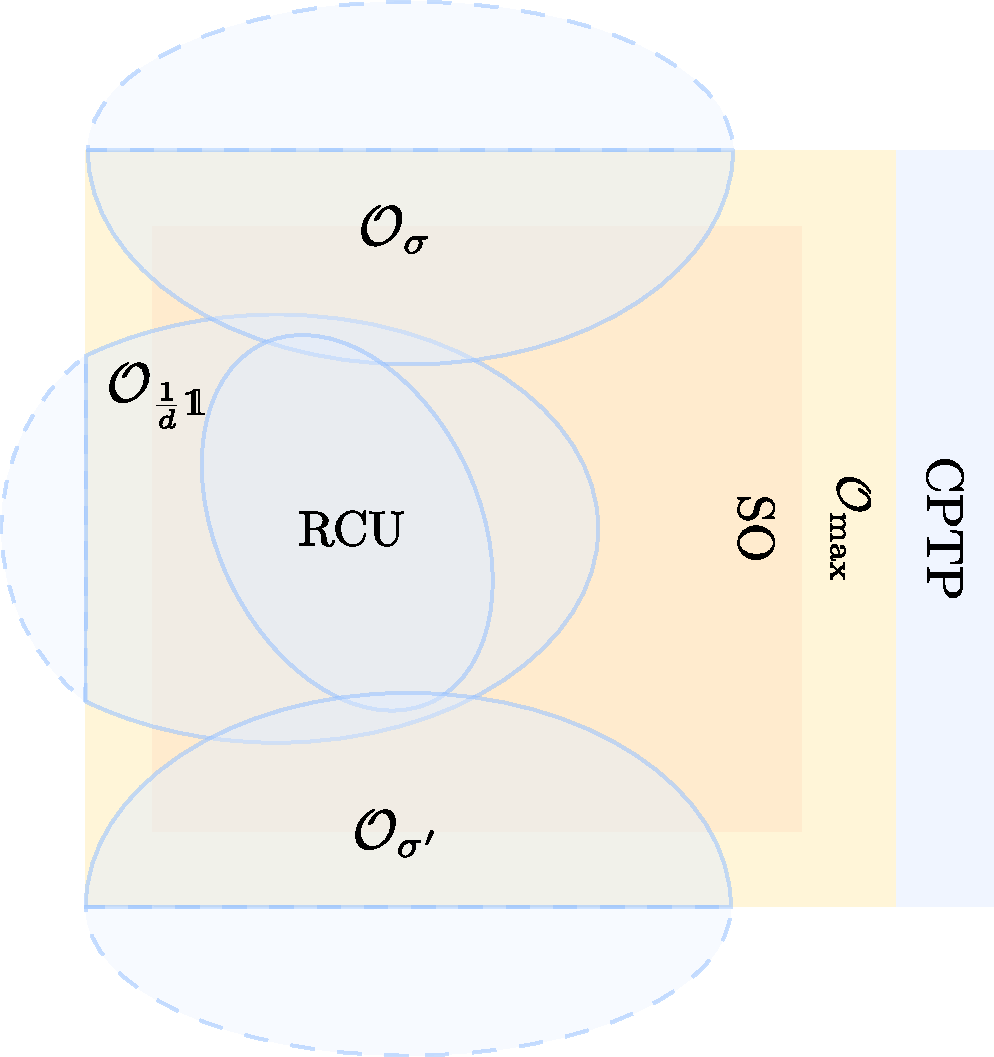
\includegraphics[scale=0.47
        ]{sections/major/operations.pdf}
    \caption{Zoo of allowed operations for magic resource theories.
    Established theories involve operations within the yellow regions, following the hierarchy $\so \subset \cspo \subset \spo \subset \Omax$.
    We introduce fragments $\O_\sigma,\ \sigma \in \F$ that cover $\Omax$ with each one extending to a set of stochastic maps that allows for $\bmd$-majorization to be used.
    }
    \label{fig:zoo}
\end{figure}

The subdivision of magic theories into $\sigma$-fragments is powerful because the pre-order $\prec_{\R'}$ of every $\sigma$-fragment is described by well-behaved majorization tools, as we establish in~\cref{sec:major}. \nick{expand}

\subsection{Majorization}\label{sec:major}

Majorization is a powerful tool that has recently found many applications in quantum information theory \nick{CITE}.
It can describes the \nick{disorder / non-uniformity} of distributions that undergo stochastic transformations.

To formally state majorization results, we first denote by $\stoch$ the set of $(d \times d)$ stochastic matrices that preserve the probability vector $\bmd$. \nick{Should we introduce notation directly in the magic setting?}
Specifically, for any $S \in \stoch$, all matrix elements are non-negative, all rows sum to $1$ and $S\bmd = \bmd$.
\iffalse
\begin{enumerate}
    \item $S_{ij} \geq 0$ for all $i, j \in \zd$;
    \item $\sum\limits_{j=1}^n S_{ij} = 1$ for all $i \in \zd$;
    \item $S\bmd = \bmd$.
\end{enumerate}
\fi
The set $\stoch$ forms a group under matrix multiplication for all $\bmd$ with positive components.

Majorization finds an important application on quantum thermodynamics in the absence of coherence.
The use of majorization in this setting provides useful intuition for our purposes.
At any given temperature $\beta$, the thermal state $\gamma_\beta$ is thermodynamically the most ordered state. 
Thermal operations are defined as operations that cannot extract energy from the Gibbs state, $\E(\gamma_\beta) = \gamma_\beta$.
Convertibility between states via thermal operations is equivalent to a stochasticity condition on the energy level populations of the states \nick{CITE}.
Roughly, the statement is that there exists a thermal operation $\E$ such that $\tau = \E(\rho)$ if and only if there exists a a matrix $S \in \stoch$ such that $\bm{q} = S\bm{p}$, where $\bm{q}, \bm{p}$ and $\bmd$ and the energy level population vectors of $\tau, \rho, \gamma_\beta$ respectively.

Drawing intuition from this setting, we can define majorization as follows.
\begin{definition}[\textbf{$\boldsymbol\bmd$-majorization}]\label{def:dmajor}
    Given $\bmx, \bmy, \bmd \in \reals^d$, such that the components of $\bmd$ are positive, $\bmy$ is said to $\bmd$-majorize $\bmx$, iff there exists a matrix $S \in \stoch$ such that $\bmx = S\bmy$.
\end{definition}
We denote this pre-order by $\bmx \prec_{\bmd} \bmy$.
If $\bmd = \frac{1}{d}\bm{1}$, the $d$-dimensional uniform distribution, then $\stoch$ is the set of doubly stochastic matrices and we retrieve the familiar notion of majorization in entanglement theory. \nick{CITE}

\nick{We need to address the non-full-rankness of states.\\
For example, the operation $\E(\rho) = \ketbra{0}$ corresponds to no $\sigma$-fragment because components of $\W{\sigma}$ are zero.\\
In such a case we can always add some $\epsilon$ amount of unital noise by mixing $\sigma$ with the maximally mixed state $\frac{1}{d}\id$. 
This ensures that all components are strictly positive and $\bmd$-majorization can be used.
There are non-full-rank states with no zeros in W.}

The pre-order $\prec_{\R'}$ of the $\sigma$-fragment $\R' = (\F, \O_\sigma)$ between $d$-dimensional states corresponds to the majorization pre-order $\prec_{\W{\sigma}}$ between their $d^2$-dimensional Wigner distributions.

\begin{theorem}
    Let $\R = (\O, \F)$ be a theory of magic.
    Suppose the state conversion $\rho \xrightarrow{\E \in \O} \tau$ is possible. 
    Then, there exists a full-rank free state $\sigma \in \F$ such that  $\W{\tau} \prec_{\W{\sigma}} \W{\rho}$.
\end{theorem}
\begin{proof}
    Suppose there exists $\E \in \O$ such that $\E(\rho) = \tau$.
    The free operation belongs to a $\sigma$-fragment, $\E \in \O_\sigma$, for some $\sigma \in \F$.
    Then, $\W{\E}\W{\rho} = \W{\tau}$ with $\W{\E} \in \stochw$, or, equivalently, $\W{\tau} \prec_{\W{\sigma}} \W{\rho}$.
\end{proof}

A visual representation of $\bmd$-majorization is provided by Lorenz curves.
Let the vector $\bmz^\downarrow$ denote a component permutation of vector $\bmz \in \reals^d$, so that its components are arranged in non-increasing order.
\begin{definition}[\textbf{Lorenz curve}]
    Let $\bmz \in \reals^d$.
    Let $\bmd \in \reals^d$ be a vector with positive components, $\pi$ a permutation mapping $(z_i/d_i) \mapsto (z_i/d_i)^\downarrow$ for all $i=1,\dots,d$ and $D = \sum_{i=1}^d d_i$.
    The Lorenz curve $L(\bmz|\bmd)$ of vector $\bmz$ is the piecewise linear curve obtained by joining the points $\{ (x_k, L_k(\bmz|\bmd)) \}_{k=1,\dots,d}$, where
    \begin{equation}\label{eq:lorenz}
        (x_k, L_k(\bmz|\bmd)) \coloneqq \left( \frac{1}{D}\sum_{i=1}^k d_{\pi(i)}, \sum_{i=1}^k z_{\pi(i)} \right) \in \mathbb{R}^2.
    \end{equation}
\end{definition}
\emph{Remark 1.} The origin $(x_0, L_0(\bmz|\bmd)) \coloneqq (0,0)$ is usually included in the curve.

\emph{Remark 2.} Components $x_k$ are rescaled by $D$ so that comparison of curves with unequal dimensions is possible.
In fact, the Lorenz curves $L(\bmz|\bmd)$ and $L(\bmz \otimes \bmd|\bmd \otimes \bmd)$, where $\otimes$ denotes the Kronecker product, are identical.

\emph{Remark 3.} Lorenz curves are always concave.

\emph{Remark 4.} If $L_d(\bmz|\bmd) = 1$ and for all $k$, $L_k(\bmz|\bmd) \leq 1$, then $\bmz$ is a probability distribution.
Lorenz curves of quasi-probability distributions in principle reach above 1.

A vector $\bmy$ $\bmd$-majorizes another vector $\bmx$  if and only if Lorenz curve $L(\bmy|\bmd)$ lies above Lorenz curve $L(\bmx|\bmd)$.
\begin{theorem}\label{thm:dmajor}
    Let $\bmx, \bmy, \bmd \in \reals^d$, such that the components of $\bmd$ are positive. 
    Then, $\bmx \prec_{\bmd} \bmy$ if and only if $L_k(\bmx|\bmd) \leq L_k(\bmy|\bmd)$ for all $k=1,2,\dots, d-1$ and $L_d(\bmx|\bmd) = L_d(\bmy|\bmd)$.
\end{theorem}
A restatement of the theorem including more equivalent conditions, along with a proof is provided in the \nick{appendix}.

An example of comparison between different Lorenz curves is illustrated in~\cref{fig:lctoy}.
\begin{figure}
    \centering
    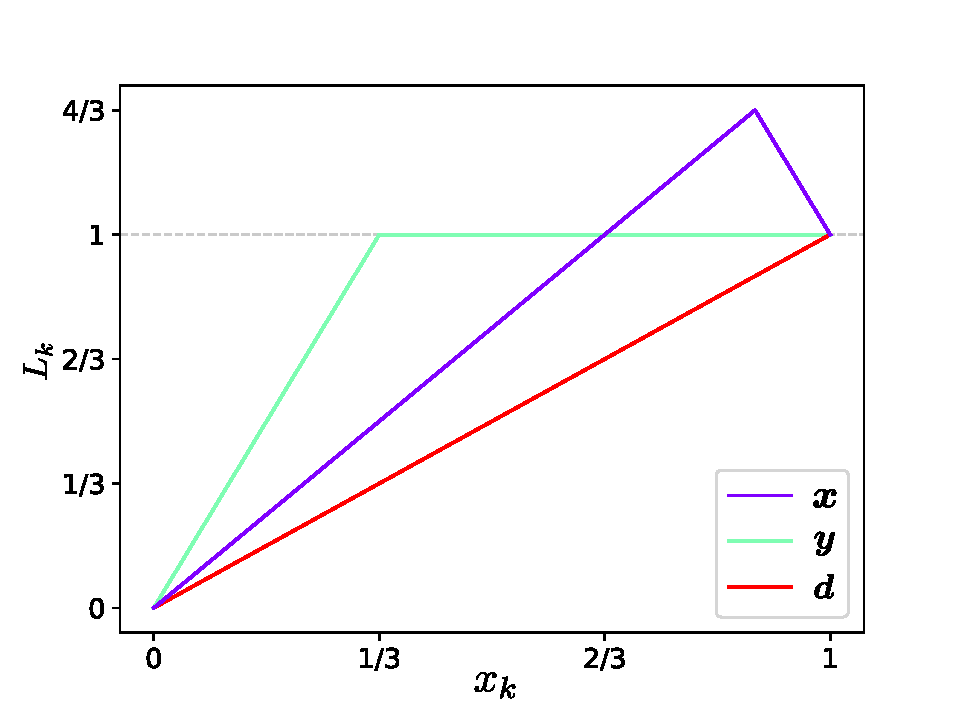
\includegraphics[height=5cm]{sections/major/lctoy.pdf}
    \caption{Example of different Lorenz curves for quasi-probability vectors under $\bmd$-majorization.
    Vectors $\bmy$ and $\bmd$ are simply probability distributions.
    The curve corresponding to vector $\bmd$ is always the line segment connecting $(0,0)$ and $(1,1)$, so that any other Lorenz curve lies above it, for example $\bmx \prec_{\bmd} \bmd$.
    Curves $L_k(\bmx|\bmd)$ and $L_k(\bmy|\bmd)$ intersect, so $\bmx \nprec_{\bmd} \bmy$ as well as $\bmy \nprec_{\bmd} \bmx$.
    \nick{Recast in terms of magic}
    }
    \label{fig:lctoy}
\end{figure}

\subsection{Set theoretic properties of magic fragments}\label{sec:propmagfrag}

\nick{May move statements around the section or in an appendix.}

\begin{theorem}\label{thm:frag}
    Let $\R = (\O, \F)$ be a magic theory. 
    The following statements hold:
    \begin{enumerate}
        \item No $\sigma$-fragment is empty.
        \item If a free operation leaves two states invariant, then it also leaves their mixtures invariant, 
        \begin{equation}
            \O_{\sigma} \cap \O_{\sigma'} \subseteq \O_{p\sigma + (1-p)\sigma'}\ \text{for all}\ p \in [0,1].
        \end{equation}
        \item Let $\E$ be a $\cptp$ operation with Wigner distribution $\W{\E}$.
        For $\R = \Rmax$ $\E \in \O_\sigma$ iff $\W{\E} \in \stochw$.
    \end{enumerate}
\end{theorem}
\begin{proof}$ $\\

    \begin{enumerate}
    \item Consider the completely depolarising \nick{replacement} map
    \begin{align}
        \E(\rho) &= \sigma \tr[\rho],\ \text{with} \\
        \W[\bmy|\bmx]{\E} &= \W[\bmy]{\sigma} \tr[\rho],
    \end{align}
    where $\sigma \in \F$. 
    Then, $\E \in \O_\sigma$.
    It can be thought as a sequence of tracing out state $\rho$ and preparing the free state $\sigma$.
    
    \item Let $\E \in \O_{\sigma} \cap \O_{\sigma'}$.
    Then $\E \in \cptp$ and corresponds to stochastic Wigner distribution $\W{\E}$ such that $\W{\E} \W{\sigma} = \W{\sigma}$ and $\W{\E} \W{\sigma'} = \W{\sigma'}$.
    Then, $\W{\E} \W{p\sigma + (1-p)\sigma'} = \W{p\sigma + (1-p)\sigma'}$ for any $p \in [0,1]$ due to the additive property~\ref{en:w4} of the Wigner distribution, implying that state $p\sigma + (1-p)\sigma'$ is also left invariant by $\E$.
    
    \item Let $\O_\sigma' \coloneqq \{ \E \in \cptp: \W{\E} \in \stochw \}$ be the described set of operations.
    
    Suppose $\E$ is in $\O_\sigma$, then $\E \in \cptp$ and $\W{\E} \in \stochw$ due to property~\ref{en:wo4} of~\cref{thm:wchannel}, hence $\O_\sigma \subseteq \O_\sigma'$.
    
    Conversely, suppose $\E \in \cptp$ with $\W{\E} \in \stochw$. 
    Then, $\W[\bmy|\bmx]{\E} \geq 0$ for all $\bmx, \bmy$, hence $\E \in \O$.
    Furthermore, $\W{\E} \W{\sigma} = \W{\sigma}$ implies $\E(\sigma) = \sigma$ using~\cref{eq:woperation} defined for any $\cptp$ operation $\E$.
    Hence, $\O_\sigma' \subseteq \O_\sigma$.
    \end{enumerate}
\end{proof}

Any free state $\sigma \in \cal{B}(\hd)$ corresponds to a $d^2$-dimensional probability distribution $\W{\sigma}$ and any free operation $\E: \cal{B}(\hd) \mapsto \cal{B}(\hd)$ corresponds to a $d^2 \times d^2$ stochastic matrix (or conditional probability distribution) $\W{\E}$.
Note that these mappings are one-to-one due to the orthogonality of the phase-point operators as an operator basis.

\emph{Remark 1.} Note that free states $\F$ are mapped onto a \emph{strict subset} of the set of probability distributions.
As a counterexample, the sharp $d^2$-dimensional probability distribution $(1, 0, \dots, 0)$ does not correspond to any qudit Wigner distribution because of the boundedness condition~\ref{en:w3} in~\cref{thm:wstate}.

\emph{Remark 2.} Similarly, not all stochastic matrices correspond to $\cpos$ operations.

As an example, consider the permutation matrix
\begin{equation}
    \Pi_X = \begin{psmallmatrix}
        0 & 1 & 0 & 0 & 0 \\
        0 & 0 & 0 & 0 & 1 \\
        0 & 0 & 0 & 1 & 0 \\
        1 & 0 & 0 & 0 & 0 \\
        0 & 0 & 1 & 0 & 0
    \end{psmallmatrix} \otimes \begin{psmallmatrix}
        0 & 0 & 1 & 0 & 0 \\
        0 & 0 & 0 & 0 & 1 \\
        0 & 0 & 0 & 1 & 0 \\
        1 & 0 & 0 & 0 & 0 \\
        0 & 1 & 0 & 0 & 0    
    \end{psmallmatrix} \in \stochw,\ d=5.
\end{equation}
It preserves the uniform distribution $\W{\frac{1}{5}\id}{}$, but it does not correspond to any completely positive operation and therefore to any $\E \in \O$, due to~\cref{thm:frag}.